\section{Experiments}\label{sec:experiments}
We compute the constants of Sections~\ref{sec:general}--\ref{sec:population} exactly for trained models. Every population $P$ is a held-out or target empirical law mixed with a uniform mass of $1\%$ over profiles and labels, which gives full support; every design is pointwise unbiased; and every reported constant is certified by primal and dual bounds that agree to a relative error of at most $10^{-4}$. Ratios are $W_\A(P)/W_{\rm branch}(P)$, the factor by which the best design of a class needs more records than the best branching design. Protocols, every per-run value and sensitivity analyses are in Appendix~\ref{app:F}.

\paragraph{Forest updates.}
On WDBC, Spambase and Ionosphere \citep{wolberg1993,spambase1999,ionosphere1989}, an old and a new random forest of twenty depth-$b$ trees are trained on disjoint records with $m\in\{6,9,12\}$ median-binarized features, and the remaining 269, 3,101 and 171 records define $P$. The contrast is the difference of the forests' predicted probabilities, so no single tree computes it and even branching falls short of complete records. Table~\ref{tab:capgrid} reports caps two to four. At cap three the best pre-committed design needs a median \nCapThreeMed{} times as many records as the best branching design (range \nCapThreeMin--\nCapThreeMax). An exact optimal two-round design recovers \nTwoForestLo--\nTwoForestHi\% of the log-gap, $1-\log(W_2/W_{\rm branch})/\log(W_{\rm fixed}/W_{\rm branch})$, in each of the \nTwoForestN{} tasks where it was computed and needs at most \nTwoForestRatioMax{} times the records of branching. Branching restricted to the forests' own trees captures a median of only \nCapThreeShare\% of the log-gap at cap three. For these ensembles the cap costs more than pre-commitment does: relative to complete records, the best fixed designs need \nCapFixLo--\nCapFixHi{} and the best branching designs \nCapBrLo--\nCapBrHi{} times as many records (medians by cap).

\begin{table}[t]
\centering
\caption{Forest updates of depth $b$ under cap $b$ (WDBC, Spambase, Ionosphere; binding tasks). Fixed/branch: exact $W_{\rm fixed}/W_{\rm branch}$, median [minimum, maximum]. Fit: median excess of the ratio realized by designs optimized on training records over the exact ratio of the same task ($^\dagger$the 15 tasks with $m=12$). Own: share of the log-gap captured when branching may use only the forests\textquotesingle{} own trees. Two: exact optimal two-round design, $W_2/W_{\rm branch}$ ($^\ddagger$five splits per cell: 45 and 15 tasks; at $b=2$ two rounds are branching). Cap: $W_{\rm fixed}$ and $W_{\rm branch}$ relative to the full-information variance.}
\label{tab:capgrid}
\footnotesize
\setlength{\tabcolsep}{2.6pt}
\begin{tabular}{rrlrrrrr}
\toprule
 & & & & & & \multicolumn{2}{c}{Cap: /full} \\
$b$ & tasks & Fixed/branch & Fit & Own & Two & fixed & branch \\
\midrule
2 & 45 & 1.31 [1.12, 1.49] & +1\% & 49\% & 1 & 4.1 & 3.3 \\
3 & 180 & 1.51 [1.14, 1.85] & +2\%$^\dagger$ & 17\% & 1.04$^\ddagger$ & 3.5 & 2.3 \\
4 & 15 & 1.24 [1.13, 1.35] & +3\% & 26\% & 1.03$^\ddagger$ & 1.4 & 1.1 \\
\bottomrule
\end{tabular}
\end{table}

\begin{table*}[t]
\centering
\caption{Screening trees on twelve items: records needed relative to branching, which asks the tree\textquotesingle s own questions and attains the full-information variance (medians over two targets and three seeds; the range is over runs). Best: optimal fixed design over all forms at the target law. Fitted: the same program on source records, evaluated at the target. Label: optimal fixed design whose form probabilities may depend on the label. Two: exact optimal two-round design (at $b=6$ the median includes certified upper bounds from feasible two-round designs for 4 runs, Table~\ref{tab:runs}). Two fit.: two-round design fitted on source records. Naive pre-committed designs with the best scores for each: U-paths, uniform over the tree\textquotesingle s question paths; U-items, uniform over all $b$-subsets of the items the rule depends on; U-all, uniform over all $\binom{12}b$ forms. $1/\rho_P^2$, $N_P$: the ends of Theorem~\ref{thm:bracket}. -- not computed.}
\label{tab:screening}
\footnotesize
\setlength{\tabcolsep}{4.6pt}
\begin{tabular}{lrrlrrrrrrrrr}
\toprule
Data, $b$ & runs & Best & [min, max] & Fitted & Label & Two & Two fit. & U-paths & U-items & U-all & $1/\rho_P^2$ & $N_P$ \\
\midrule
BRFSS, 3 & 6 & 1.00 & [1.00, 1.34] & 1.04 & 1.00 & 1.00 & 1.00 & 1.03 & 1.00 & 15.8 & 1.00 & 1.5 \\
BRFSS, 4 & 6 & 1.49 & [1.00, 1.75] & 1.57 & 1.48 & 1.00 & 1.01 & 1.80 & 2.30 & 21.7 & 1.18 & 3.3 \\
BRFSS, 5 & 6 & 1.35 & [1.18, 1.54] & 1.42 & 1.35 & 1.00 & 1.01 & 1.72 & 2.04 & 12.9 & 1.08 & 5.4 \\
BRFSS, 6 & 6 & 1.58 & [1.42, 1.98] & 1.68 & -- & $\le$1.05 & -- & 2.30 & 4.18 & 11.1 & 1.13 & 10.5 \\
Thyroid, 3--6 & 24 & 1.00 & [1.00, 1.00] & 1.04 & 1.00 & 1.00 & 1.04 & 1.20 & 1.00 & 4.9 & 1.00 & 3.6 \\
\bottomrule
\end{tabular}
\end{table*}


\paragraph{Screening questionnaires.}
A depth-$b$ screening tree asks at most $b$ questions per person, so a validation study under the same burden must respect the cap. We train class-balanced CART trees on twelve yes/no items of the CDC Diabetes Health Indicators, derived from the Behavioral Risk Factor Surveillance System (BRFSS; 253,680 respondents, target diabetes or prediabetes) \citep{cdcdiabetes2017}, and on twelve binarized thyroid items (7,200 patients, abnormal function) \citep{quinlan1986thyroid}, and validate them on a disjoint random half or on respondents of the other sex. Table~\ref{tab:screening} summarizes the runs and Table~\ref{tab:runs} lists each one.

\emph{The price of pre-commitment.} On BRFSS the best pre-committed design needs a median \nScreenBestLo--\nScreenBestHi{} times as many respondents at caps four to six (\nScreenRunLo--\nScreenRunHi{} over runs). On thyroid, and for the BRFSS trees that use at most $b$ items, one form explains the whole target ($\rho_P^2=1$) and pre-commitment costs nothing. Letting the form probabilities depend on the label, or on the label and sex, lowers the ratio by at most \nLabelMax\% and \nStratMax\%, so the cost is not an artifact of label-blind forms.

\emph{What optimization of the forms buys.} A collector who knows the rule would not randomize over items it never uses. Uniform randomization over the tree's own question paths, with the best scores for that design, needs \nUpsLo--\nUpsHi{} times the records of branching at caps four to six, a median \nUpsOverMed\% (at most \nUpsOverMax\%) more than the optimized design; uniform randomization over all $b$-subsets of the items the rule depends on needs \nUitLo--\nUitHi{} times (median \nUitOverMed\% more), and uniform randomization over all forms, the default of multipurpose matrix sampling, \nUnifLo--\nUnifHi{} times. For a 95\% interval of $\pm2$ accuracy points at $b=5$, branching needs about \nSsBranch{} respondents, optimized forms \nSsFixed{} and uniform path forms \nSsUps{} (medians). Restricting the optimized design to the tree's path sets loses a median \nPsGapMed\% (at most \nPsGapMax\%) over the \nPsGapN{} runs with a gain; the lower end $1/\rho_P^2$ of the bracket is below the realized ratio by a median factor \nLowUnder{} and the upper end $N_P$ above it by \nNpOver.

\emph{One adaptive round.} Of the \nScreenGainN{} BRFSS runs with a gain, \nGainComputable{} have trees that a two-round interview with at most $b$ questions computes exactly, so a second round removes the whole cost. For \nGainExactNon{} others the optimal two-round design was computed and recovers at least \nGainExactNonMin\% of the log-gap (ratio at most \nScreenTwoMax). For the remaining \nTwoBounded{}, all at $b=6$, column generation was stopped after one hour; the feasible two-round designs found by then need between \nTwoBoundMin{} and \nTwoBoundMax{} times the records of branching, so the second round recovers at least \nTwoBoundRec\% there. A two-round design fitted on source records needs a median \nScreenTwoFitMed{} (at most \nScreenTwoFitMax) at $b\le5$, whereas the heuristic of following the root question and then the best fixed form recovers only \nHeurLo--\nHeurHi\%. All of this is far from the worst case of Theorem~\ref{thm:rounds}.

\begin{figure}[t]
\centering
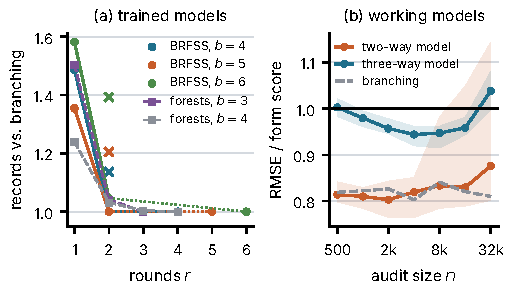
\includegraphics[width=\columnwidth]{figures/v16_rounds.pdf}
\caption{(a) Records needed relative to branching as a function of the number of rounds ($r=1$: fixed forms; $r=b$: branching): optimal $r$-round designs for BRFSS screening trees (median over targets and seeds; at $b=6$, $r=2$ the median includes upper bounds) and forest updates (median over tasks); crosses mark the heuristic second round of following the root question. (b) RMSE of log-linear working models, and of branching, relative to the design-based form score on the same fitted-form records, against the audit size (median over \nCurveTrees{} BRFSS trees; bands: quartiles).}
\label{fig:rounds}
\end{figure}

\paragraph{Deployable designs.}
The ratios above compare designs tuned to the target law. Fixed designs fitted on 20,000 source records need a median \nFitMed\% (at most \nFitMax\%) more records and remain exactly unbiased. Without a reference, the design can be learned from a pilot of the audit itself (Proposition~\ref{prop:selfcal}), and the pilot must be charged. With a quarter of the records used as a pilot on the tree's paths and scored by cross-fitting, the all-in price of pre-commitment for $N=4{,}000$ records is \nAllInFourc{} at $b=4$ and \nAllInFivec{} at $b=5$, against \nPilotFourBest{} and \nPilotFiveBest{} for the oracle designs; for $N=8{,}000$ it is \nAllInFourd{} and \nAllInFived{} (medians, Table~\ref{tab:pilot}). At $b=6$ a pilot of 2,000 is too small for the \nPilotSixCells{} cell masses (all-in \nAllInSixd{} against \nPilotSixBest), and a reference is needed.

\paragraph{Scale and reuse.}
With all 21 BRFSS variables the form program has 5,985 forms at $b=4$ and the cube $2^{21}$ profiles; the solver certifies the optimal fixed design in a median of \nScaleMin{} minutes on one core (the trees are those of the twelve-item study; Appendix~\ref{app:scale}). An optimized design is tailored to one rule: scoring another screening tree on records collected for the first needs between \nReuseMin{} and \nReuseMax{} times the records of branching. If the rules are known in advance, one shared design can serve them: the fixed design that minimizes the summed ratios of three trees costs each a median \nJointPenMed\% (at most \nJointPenMax\%) more than its own optimum (Appendix~\ref{app:reuse}).

\paragraph{Design-based versus model-based estimation.}
\nModelParagraph

\paragraph{Order effects.}
If the last of $b$ answers flips with probability $0.1$ and earlier ones proportionally less often, an illustrative response model, the median absolute bias on BRFSS at $n=1000$ is \nPosBranch{} branching standard errors for branching and \nPosFit{} for the fitted form, comparable to the sampling gains above (Appendix~\ref{app:measurement}).
